\chapterimage{chapter_head_1.pdf} 
\chapter{Entrada/Salida en la NDS}

Este capítulo explica como funciona el sistema de entrada y salida de la consola Nintendo DS. La lista de ejercicios y el tiempo estimado (en minutos) para su realización se muestran en la Tabla \ref{c9_tab:ejercicios}.

\begin{table}[t]
	\centering
	\caption{Ejercicios del capítulo y tiempo estimado para su realización.}
	\begin{tabular}{|c|c||c|c|}
		\hline 
		Ejercicio & Tiempo & Ejercicio & Tiempo\\ 
		\hline 
		9.1 & 5'  & 9.6  & 5'  \\ 
		9.2 & 10' & 9.7  & 10' \\ 
		9.3 & 15' & 9.8  & 15' \\ 
		9.4 & 5'  & 9.9  & 15' \\ 
		9.5 & 15' & 9.10 & 25' \\ 
		\hline 
	\end{tabular} 
	\label{c9_tab:ejercicios}
\end{table}


% -------------------------------------------------------------------------
% -------------------------------------------------------------------------
\section{Introducción}
La videoconsola Nintendo DS dispone de una amplia variedad de periféricos muy sencillos que permiten la interacción con el usuario. Los más destacados son:

\begin{itemize}
	\item Altavoces estéreos que cuentan con 16 canales de audio independientes.
	\item Dos pantallas LCD  de 3 pulgadas. La pantalla inferior utiliza tecnología táctil.
	\item Varios temporizadores que  pueden ser utilizados por una aplicación o un juego para definir diferentes respuestas dependiendo del tiempo.
	\item Un conjunto de botones que realizan diversas funciones de teclado.
\end{itemize}

En este capítulo se describirán fundamentalmente las características de los botones y los 
temporizadores, así como la gestión de interrupciones que permite realizar operaciones de E/S en la Nintendo DS empleando los periféricos citados. 

\section{Botones}
El conjunto de botones que tiene la Nintendo DS constituyen un sencillo teclado que permite hacer operaciones de entrada muy simples, tal y como se muestran en la Figura \ref{fig:c9_botones-teclado}. Esta figura muestra, además de todos los  botones que tiene la Nintendo DS, qué procesador gestiona a cada uno de los  periféricos. 

\begin{figure}[h]
	\centering
	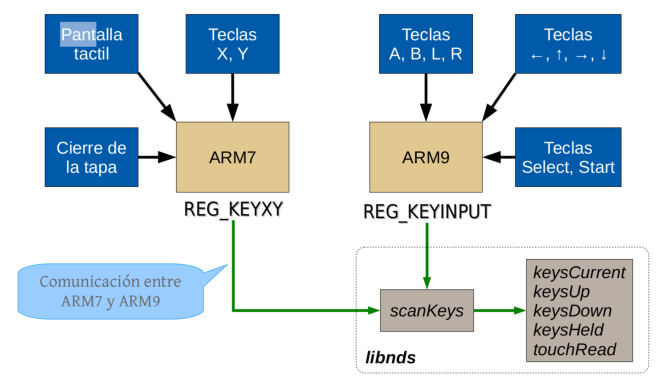
\includegraphics[height=7cm]{./Figuras/C9/c9_botones_teclado.PNG}
	\caption{Botones en la Nintendo NDS}
	\label{fig:c9_botones-teclado}
\end{figure}

La gestión de las operaciones se realiza a través de dos registros: \textit{REG\_KEYCNT} y \textit{REG\_KEYINPUT}. La figura~\ref{fig_p2_c2_registros-teclado} muestra el significado de cada uno de los  bits de ambos registros, donde cada uno de ellos representa un botón.

\begin{figure}[h]
	\centering
	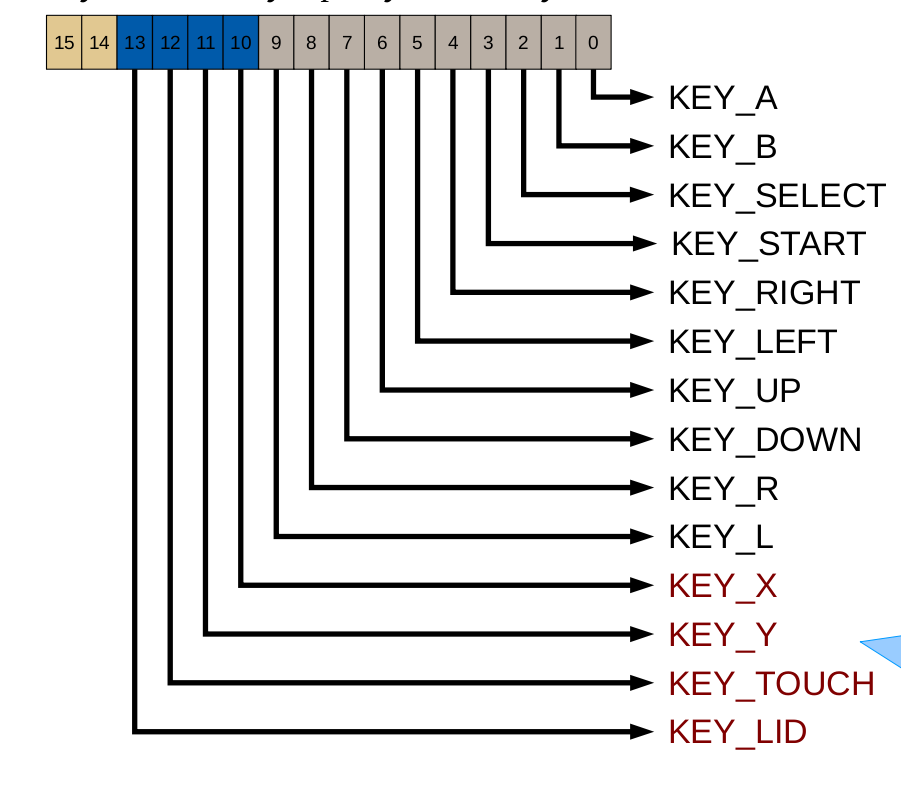
\includegraphics[height=7cm]{./Figuras/C9/c9_registros-teclado.PNG}
	\caption{Significado de los bits de los registros de los botones}
	\label{fig_p2_c2_registros-teclado}
\end{figure}

\begin{itemize}
	\item \textit{REG\_KEYCNT}: es el \textit{Registro de control} y permite habilitar o enmascarar la interrupción asociada con la pulsación de un botón. Si el bit está a 1, cuando se pulsa dicho botón se activará la petición de interrupción. En caso contrario, no se activará.
	Además de los bits para cada botón, este registro de control para las interrupciones generadas por los botones tiene dos bits específicos:
	\begin{itemize}
		\item El bit 14 permite enmascarar de forma general todas las interrupciones de los botones. Si este bit está a 0, no se activará la petición de interrupción cuando se pulse cualquier botón, aunque hubiera bits a 1 en alguno de los bits correspondientes a los botones.
		\item El bit 15 sirve para que las interrupciones se produzcan por la pulsaci\'on de un solo bot\'on (cuando el bit est\'a a 0), o de varios botones a la vez (cuando est\'a a 1). En este \'ultimo caso, la interrupci\'on se genera cuando est\'en pulsados a la vez todos los botones que tengan un 1.
	\end{itemize}
	Este registro está mapeado en la dirección de memoria \textit{0x4000132}.
	\item \textit{REG\_KEYINPUT}: Es el \textit{Registro de datos}. Almacena los botones pulsados. Pone a 0 el bit del botón que ha sido pulsado. Cuando se lee dicho registro el valor del bit vuelve  al valor inicial a 1. La disposici\'on de los bits del 0 al 13 es la misma que la descrita en el registro \textit{REG\_KEYCNT}.
	Este registro está mapeado en la dirección de memoria \textit{0x4000130}.
\end{itemize}

% -------------------------------------------------------------------------
% -------------------------------------------------------------------------
\section{Temporizadores}
Un temporizador contiene un contador programable que cuenta de forma ascendente o descendente  a la velocidad que le marca la frecuencia de trabajo. La cuenta, la dirección del conteo y el divisor de frecuencia, en la mayoría de los dispositivos, es programable. La característica  más importante de estos dispositivos es que cuando alcanzan la cuenta final  pueden solicitar una interrupción al procesador, siempre y cuando la tengan habilitada.  Por ejemplo, supongamos un temporizador que cuenta de forma ascendente desde el valor que se carga en el contador hasta el máximo de cuenta que puede alcanzar. Sea 255 (tiene 8 bits) el valor  máximo  y  20 el valor inicial. El contador inicia la cuenta ascendente en el momento que se le da la orden de inicio  desde 20 hasta  255  y cuando alcanza ese valor solicitará una interrupción al procesador. El tiempo transcurrido entre ambas cuentas  depende de la frecuencia del contador. 

La Nintendo DS dispone de 8 temporizadores de 16 bits: cuatro en el ARM7 y cuatro en el ARM9. En los temporizadores que tiene la Nintendo DS, el contador siempre contará  de forma ascendente desde la cuenta cargada (programable)  hasta la máxima que puede alcanzar el contador (fijada por el número de bits, 16). En este caso, la programación del temporizador consistirá en establecer el valor inicial de la cuenta, el divisor de frecuencia, habilitar la interrupción y enviar la orden de  inicio del contador. El temporizador  solicitará una interrupción al procesador cuando alcanza la cuenta máxima.

La gestión de las operaciones con los  temporizadores se lleva a cabo mediante dos registros:

\begin{itemize}
	\item \textit{TIMER\_CR(n)} (\textit{Registro de control}): Se utiliza para programar el modo de trabajo del temporizador, donde \textit{n} indica cuál se está utilizando de los cuatro posibles (0,1,2,3). En este registro se escribe la siguiente información de control:
	\begin{itemize}
		\item Divisor de frecuencia utilizado: 1, 64, 256, 1024.
		\item Modo de trabajo: cascada o no. Es decir, si conectamos varios temporizadores en cadena para ampliar el rango de la cuenta. 
		\item Habilitación/enmascaramiento de  la interrupción: 1 habilitada, 0 enmascarada.
		\item Habilitación del temporizador: si se pone a 1 el bit correspondiente, el temporizador empieza la cuenta a partir de este momento.
	\end{itemize}
	En la figura~\ref{fig_p2_c2_timer-control} se muestra la distribución de los bits del registro \textit{TIMER\_CR(n)} para su programación. 
	\item \textit{TIMER\_DATA(n)} (\textit{Registro de datos}): Almacena la cuenta de inicio. 
\end{itemize}


\begin{figure}[h]
	\centering
	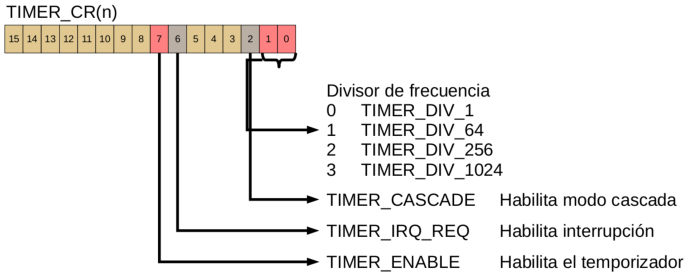
\includegraphics[height=5.5cm]{./Figuras/C9/c9_timer.PNG}
	\caption{ Campos de bits de \textit{TIMER\_CR(n)}}
	\label{fig_p2_c2_timer-control}
\end{figure}

Los registros \textit{TIMER\_DATA(0)} y \textit{TIMER\_CR(0)} están mapeados en las direcciones de memoria 0x4000100 y 0x4000102, respectivamente; los registros   \textit{TIMER\_DATA(1)} y \textit{TIMER\_CR(1)} en las direcciones de memoria 0x4000104 y 0x4000106, respectivamente; y así sucesivamente. 

% -------------------------------------------------------------------------
% -------------------------------------------------------------------------
\section{Gestión de interrupciones en el procesador}
El controlador de interrupciones del procesador ARM que se encarga de la gestión de interrupciones dispone de varios registros: 

\begin{itemize}
	\item \textit{Registro maestro de interrupciones (IME)}: Es un registro de 16 bits, cuya función es la de permitir o no que se produzcan interrupciones. En la biblioteca \textit{libnds} es el registro \textit{REG\_IME} y está mapeado en memoria en la dirección \textit{0x4000208}.
	%    
	\item \textit{Registro de activación de interrupciones (IE)}: Es un registro de 32 bits que indica qué interrupciones se quieren gestionar. Cada bit activa o desactiva un tipo de interrupción (no todos se usan). En la biblioteca \textit{libnds} es el registro \textit{REG\_IE} y está mapeado en memoria en la dirección \textit{0x4000210}.  
	%
	\item  \textit{Registro de petición de interrupciones (IF)}: Es un registro de 32 bits en el que se pone a 1 el bit del tipo de interrupción que ha solicitado para interrumpir la CPU. En la biblioteca \textit{libnds} es el registro \textit{REG\_IF} (de 32 bits) y está mapeado en memoria en la dirección \textit{0x4000214}. 
\end{itemize}

Aunque la Nintendo DS puede gestionar  una amplia variedad de interrupciones hardware, las de E/S son un caso particular. Se utilizan para avisar al procesador de que el periférico  requiere su atención. 

En este capítulo sólo vamos a trabajar con dos tipos principales:
%
\begin{itemize}
	\item Interrupciones para los temporizadores: \textit{IRQ\_TIMER0, IRQ\_TIMER1, IRQ\_TIMER2, e  IRQ\_TIMER3}. Cuando el contador del temporizador 0, 1, 2 ó 3  alcanza la cuenta máxima se activará la interrupción correspondiente.
	%
	\item Interrupciones de los botones de la Nintendo DS: \textit{IRQ\_KEYS}. Cuando se pulsa alguno de los botones se activará esta interrupción.
\end{itemize}

El procesador de la  consola Nintendo DS  utiliza el direccionamiento  {\bf E/S mapeado en memoria} para asignar direcciones a los registros de los controladores. Esta técnica consiste en asignar a estos registros direcciones del mapa de direcciones de memoria y se realizan operaciones de lectura o escritura con las instrucciones que permiten el acceso a memoria.

Las  interrupciones son {\bf vectorizadas}. Esto quiere decir que durante la fase de procesamiento de una interrupción, la dirección de inicio de la RTI será enviada al procesador. Estas direcciones se almacenarán en una tabla en memoria y se enviará al procesador cuando la necesite. Esta tabla contiene todos los vectores de interrupción (direcciones de inicio de las RTIs) y que se identifica por el índice, es decir, posición que ocupan en dicha tabla.

El entorno de programación que estamos utilizando dispone de una  biblioteca  \textit{libnds} que contiene un conjunto de funciones que  facilita la programación de las operaciones de E/S en la Nintendo  DS y, en particular, la gestión mediante interrupciones. Las principales funciones son:

\begin{itemize}
	\item \textit{irqSet}: se utiliza para definir la rutina de tratamiento de interrupción que  gestiona una interrupción. Con esta llamada  se inicializa la tabla de interrupciones con la dirección de inicio. Esta función tendrá dos parámetros: la interrupción y el nombre de la rutina de tratamiento. 
	%
	\item \textit{irqEnable}: se utiliza para habilitar las interrupciones en el procesador. Esta función tiene como  parámetros la lista de interrupciones a habilitar separadas por el símbolo |. 
	%
	\item \textit{irqDisable}: sirve para enmascarar una interrupción en el procesador. A esta función se le pasa como parámetros la lista de interrupciones que se quieren enmascarar separadas por el símbolo |.
	%
	\item \textit{irqClear}: permite enmascarar interrupciones y además, también, las elimina de la tabla de interrupciones. Se le pasa como parámetro tantas interrupciones como se quieran eliminar. 
\end{itemize}

% -------------------------------------------------------------------------
% -------------------------------------------------------------------------
\section{Entrada de datos utilizando los botones en la Nintendo DS}
En este apartado se van a describir algunos ejemplos muy  sencillos  en los que se van a realizar operaciones de entrada utilizando los botones y temporizadores. Su gestión se realizará por consulta de estado e interrupciones. 

% -------------------------------------------------------------------------
% -------------------------------------------------------------------------
\subsection{Consulta de estado}
Como se ha descrito previamente, es una técnica muy sencilla para la gestión de la E/S.
Consiste en implementar una espera hasta que se conozca que se ha realizado una entrada. Cuando se detecta se recoge el dato introducido. 

Este programa muestra un posible ejemplo de implementación:  
\begin{small}
	\begin{verbatim}
	Leer estado periférico
	while (! preparado) {  //bucle de espera
	Leer estado periférico  // hasta preparado
	}
	Recoger dato
	\end{verbatim}
\end{small}

Como se muestra en el código, el bucle de espera se basa en la comprobación de la condición \textit{preparado}. Su implementación dependerá de las características de funcionamiento del periférico. En el caso de los botones de la Nintendo DS, el registro \textit {REG\_KEYINPUT} tiene un bit para cada  botón y que cuando se pulsa, este bit se pone a 0. Cuando se lee dicho registro  se vuelve a poner a 1. Leyendo este registro se puede conocer en qué instante se ha producido la pulsación de un botón.

\begin{example}
Veamos un ejemplo concreto, \textit{consulta\_estado.c}, en el que se espera la pulsación del botón A. El siguiente código muestra la implementación:

\begin{lstlisting}
#include <nds.h>
#include <stdio.h>

int main(void)
{
  consoleDemoInit();
  while(1) 
  {
    while (REG_KEYINPUT != 0x03FE)
      iprintf("\x1b[6;0H Esperando Boton A       ");
    iprintf("\x1b[6;0HBoton A pulsado             ");
    swiWaitForVBlank();
  }
}
\end{lstlisting}
\end{example}

En este programa se ha implementado un  bucle, etiquetado como \textit{bucle de espera}, que el procesador estará ejecutando  mientras se cumpla la condición, es decir, mientras el bit 0 del registro \textit{REG\_KEYINPUT} sea 1. Esta condición será falsa cuando este bit sea 0 y esto se produce cuando se pulsa el botón A de la NDS. El procesador espera en este bucle hasta que se pulse dicho botón. Cuando esto ocurre contin\'ua con la ejecución. Esto se repite de manera indefinida.

\begin{exercise}
Crea un proyecto con el código del ejemplo anterior y comprueba que funciona correctamente.
\end{exercise}

\begin{exercise}
Modifica el programa anterior para que se espere a la pulsación del botón B en vez del A.
\end{exercise}

\begin{exercise}
Crea un programa que cuente el número de veces que se pulsan cada uno de los botones A, B, UP y DOWN.
\end{exercise}

% -------------------------------------------------------------------------
% -------------------------------------------------------------------------
\subsection{Interrupciones}
En esta técnica, el periférico avisa al procesador que está preparado para llevar a cabo la transferencia de información. Para llevar a cabo su gestión es necesario:

\begin{itemize}
	\item  inicialización del controlador, 
	\item  inicialización del  procesador, 
	\item diseño de la rutina de tratamiento de la interrupción (RTI), 
	\item actualización  de la tabla de direcciones para que durante la fase de procesamiento de una interrupción esta información se envíe al procesador para que realice el salto a la RTI, y 
	\item diseño de la RTI para gestionar esta interrupción.
\end{itemize}

\begin{example}
Para ver cómo se implementa esta gestión en la Nintendo DS se muestra un ejemplo sencillo (\textit{interrupciones.c}), donde se describe cómo se llevan a cabo todas estas acciones. El programa captura la pulsación del botón A y muestra el mensaje del botón pulsado: 

\begin{lstlisting}
#include <nds.h>
#include <stdio.h>
int contador = 0;

void int_boton() 
{
  if (REG_KEYINPUT == 0x03FE)
  {
    iprintf("\x1b[1;0H Boton A Pulsado");
    contador = 0;
  }
}

int main(void)
{
  irqSet(IRQ_KEYS,int_boton);
  irqEnable(IRQ_KEYS); 
  REG_KEYCNT = 0x4001; 
  
  consoleDemoInit();
  while (1)
  { 
    contador ++;
    iprintf("\x1b[1;0HPulsa A                ");
    iprintf("\x1b[14;0HContador = %04i", contador);

    swiWaitForVBlank();
  }
}
\end{lstlisting}
\end{example}

Este código contiene el programa principal (\textit{main}) y la rutina que trata la interrupción (\textit{int\_boton}). Las operaciones que se realizan en el programa principal son las siguientes:

\begin{enumerate}
	\item   Asignar la RTI \textit{int\_boton} que gestiona la interrupción de los botones (\textit{IRQ\_KEYS}) mediante la función \textit{IrqSet}. Esta rutina se almacena en memoria y actualiza la tabla de interrupciones con la dirección de inicio de esta rutina. Esta dirección se proporcionará al procesador durante el procesamiento de una interrupción. 
	%
	\item Inicialización en el procesador: Habilitar la interrupción de los botones en el procesador (\textit{IRQ\_KEYS}) mediante \textit{irqEnable}.
	%
	\item Inicialización del controlador: Habilitar la interrupción del botón A en el controlador. Esto se realiza poniendo a 1 el bit 0 del registro \textit{REG\_KEYCNT}. De esta forma cuando se pulse el botón A se activará la interrupción \textit{IRQ\_KEYS}. 
	%
	\item A continuación el programa principal implementa un bucle infinito. El procesador estará ejecutando dicho bucle, y cuando se pulse el botón A, interrumpe su ejecución, atiende la interrupción y retorna. 
\end{enumerate}

Por otro lado, la RTI codifica las acciones que se tienen que ejecutar cuando se pulsa algún  botón. La tarea principal de la RTI es identificar qué botón ha solicitado la interrupción y muestra el mensaje del botón pulsado.

\begin{exercise}
	Comprueba que el programa anterior funciona correctamente.
\end{exercise}

\begin{exercise}
Modifica el programa realizado en el Ejercicio 9.3 para usar interrupciones en vez de consulta de estado. Puedes partir del ejemplo anterior.
\end{exercise}

% -------------------------------------------------------------------------
% -------------------------------------------------------------------------
\subsection{E/S con el temporizador por interrupciones}

En este apartado se muestra cómo se trabaja con el temporizador. 

\begin{example}
A continuación se muestra un ejemplo de su funcionamiento (\textit{temporizador.c}). Se va a utilizar para contabilizar los segundos transcurridos desde que se inicializa. 

\begin{lstlisting}
#include <nds.h>
#include <stdio.h>
int contador = 0;

void int_timer() 
{
  contador ++;
}

int main(void) 
{
  consoleDemoInit();
  irqEnable(IRQ_TIMER0);
  irqSet(IRQ_TIMER0,int_timer); 

  TIMER_DATA(0)=32764; 
  TIMER_CR(0) = TIMER_DIV_1024 | TIMER_ENABLE | TIMER_IRQ_REQ ;
  while(1) 
  {
    iprintf("\x1b[12;2H%2i", contador);
    swiWaitForVBlank();
  }
}
\end{lstlisting}
\end{example}

Este código contiene el programa principal (\textit{main}) y la rutina que trata la interrupción (\textit{int\_timer}). Las operaciones que se realizan en el programa principal son las siguientes:

\begin{enumerate}
	\item Inicialización en el procesador: Habilitar las interrupciones del temporizador 0 \textit{IRQ\_TIMER0} en el procesador.
	%
	\item Actualización de  la tabla de vectores de interrupción para que la interrupción del temporizador  sea gestionada por la rutina \textit{int\_timer}. 
	%
	\item Inicialización del temporizador:
	\begin{itemize}
		\item Inicialización del temporizador: Cargar el valor inicial de la cuenta en el registro \textit{TIMER\_DATA(0)} del temporizador para que sea posible contabilizar \textit{T} segundos. El temporizador trabaja a una frecuencia base de 33.554 Mhz (\textit{frec\_base}). Para fijar este valor inicial,  \textit{cuenta\_inicial}, y la frecuencia de trabajo, \textit{frec\_trabajo}, se utilizará la siguiente fórmula:
		
		\begin{verbatim}
		cuenta_final = 65.536 
		(cuenta maxima del contador de 16 bits)
		frec_base =33.554 MHz
		frec_trabajo = frec_base/divisor 
		T_ciclo = 1/frec_trabajo
		T = (cuenta_final-cuenta_inicial)*T_ciclo
		cuenta_inicial = cuenta_final - T * frec_trabajo
		\end{verbatim}
		
		En este caso, si se desea generar una interrupción por segundo, \textit{T} será 1, y el valor que se obtiene para \textit{cuenta\_inicial} será 32.768. Por tanto se asigna este valor a \textit{TIMER\_DATA(0)}.
		%
		\item Habilitación de la interrupción del temporizador:  Consiste en definir el divisor de frecuencia, habilitar la interrupción y dar la orden de inicio. Esta información se especifica en el registro \textit{TIMER\_DATA(0)}. 
		En la configuración del registro de control {\textit TIMER\_CR(0)} se indica que se emplea un división de frecuencia de 1024, que se habilita el temporizador (\textit{TIMER\_ENABLE}) y que se genera una interrupción cuando se alcanza la cuenta máxima (\textit{TIMER\_IRQ\_REQ}). Con esta configuración se consigue generar una interrupción por segundo (aproximadamente).
		\end {itemize}
		%    
		\item En el programa principal se estará ejecutando un bucle infinito que muestra la variable segundos, que contabiliza los segundos transcurridos. A medida que se produce la interrupción del \textit{timer}, la gestiona y continúa con la ejecución.  
	\end{enumerate}
	
	La RTI \textit{int\_timer} incrementa la variable segundos. El valor de esta variable se corresponde con los segundos transcurridos desde el comienzo de la ejecución, puesto que el temporizador está programado para generar una interrupción cada segundo. 

\begin{exercise}
Comprueba el funcionamiento del programa anterior.
\end{exercise}

\begin{exercise}
Cambia el programa anterior para que el contador se incremente cada medio segundo.
\end{exercise}

\begin{exercise}
Cambia el programa anterior para que existan dos contadores, uno que se incrementará cada segundo y otro cada 2.
\end{exercise}

% -------------------------------------------------------------------------
% -------------------------------------------------------------------------
% -------------------------------------------------------------------------
% -------------------------------------------------------------------------
\section{Ejercicios avanzados}
\begin{exercise}
	Modifica el programa carreras de caballos para que el paso del tiempo se realice con interrupciones. Puedes partir de la solución proporcionada por el profesor.
\end{exercise}

\begin{exercise}
Realiza un programa que cada segundo incremente una variable por 1, empezando por el valor 0. El valor de esta variable se deberá mostrar por pantalla usando una cadena de caracteres. Para ello se deberá usar un temporizador controlado mediante interrupciones. Además, cuando se pulse el botón A, se cambiará la frecuencia de actualización para que sea cada 2 segundos (1 interrupción cada 2 segundos). Si se pulsa el botón B, la frecuencia será cada 0.5 segundos (2 interrupciones por segundo). Si se pulsa el botón UP la frecuencia volverá a ser cada segundo. Por último, si se pulsa el botón DOWN, la cuenta se reiniciará a cero.
\end{exercise}


